\documentclass{beamer}

\usetheme{Madrid}

\usepackage{lipsum}
\usepackage{multicol}
\usepackage{listings}
\usepackage{multirow}


% Define a custom color
\definecolor{backcolour}{rgb}{255,255,255}
\definecolor{codegreen}{rgb}{0,0.6,0}

% Define a custom style
\lstdefinestyle{myStyle}{
    backgroundcolor = \color{backcolour},   
    commentstyle = \color{codegreen},
    basicstyle=\linespread{0.4}\tiny,
    breakatwhitespace=false,         
    breaklines=true,        
    keepspaces=true,                               
    showspaces=false,                
    showstringspaces=false,
    showtabs=false,                  
    tabsize=2,
}

% Use \lstset to make myStyle the global default
\lstset{style=myStyle}


\usepackage{graphicx}
\usepackage{listings}
\usepackage{verbatim}
\linespread{1.5}
\usepackage{pgfplots}
\usepackage{tikz}

\usepackage{amsmath, amsthm, amssymb, latexsym}

%\newtheorem{definition}{Definition}

\newcommand{\pathtoimages}{/Users/charlesrambo/Desktop/Bootcamp24/Images}

\title{UCLA Anderson Math Bootcamp}
\author{Charles Rambo}
\institute{UCLA Anderson}
\date{2024}
\location{Los Angeles, California}


\begin{document}
\input{systempreamble}

\frame{\titlepage}

\begin{frame}[allowframebreaks]

\frametitle{Table of Contents}
\tableofcontents
\end{frame}

\section{About Me}

\begin{frame}
\begin{center}
\Huge About Me
\end{center}
\end{frame}

\begin{frame}
\frametitle{About Me}

\begin{itemize}
\item \email{charles.tutoring@gmail.com}
\item \url{github.com/charlesrambo}
\item \url{linkedin.com/in/charlesrambo}
\end{itemize}
Please email your questions to me at my gmail account. Also, please feel free to connect with me on LinkedIn!

\end{frame}

\begin{frame}
\frametitle{Education}

MFE from UCLA in 2020\\

BA in Mathematics from UC Berkeley in 2009
\end{frame}

\begin{frame}
\frametitle{Experience}
\small

SSI Investment Management\\
Portfolio Research Analyst (3 years)
\begin{itemize}
\item Firm specializes in convertible securities
\item I do valuation, credit, equity, and portfolio construction from a quantitative perspective.
\end{itemize}

Rambo Tutoring (Self-Employed)\\
Math tutor and author (10 years)
\begin{itemize}
\item Did tutoring for Precalculus, Calculus, linear algebra, differential equations, statistics, probability, and more!
\item Wrote study material as well! Check out my stuff on Amazon.com!
\end{itemize}
\end{frame}

\section{How the Course Works}

\begin{frame}
\begin{center}
\Huge How the Course Works
\end{center}
\end{frame}

\begin{frame}
\frametitle{How the Course Works}
\begin{itemize}
\item Videos emailed out
\item Notes and homework posted at \url{github.com/charlesrambo/math_bootcamp_24}
\item Grade of 70\% or better to pass
\item No exams
\end{itemize}
\end{frame}

\begin{frame}
\frametitle{Homework}
\small
\begin{itemize}
\item Can work in teams of up to four people
\item Make sure everybody's name is on the homework when you submit
\item Email homework solutions to me at \email{charles.tutoring@gmail.com}
\item Homework will be math problems which require some programming
\item Please submit as an html or pdf file; no screenshots, ipynb, or py files please
\item I look over the code but I don't run it so more important to make things readable than runable
\item Due dates posted on homework
\item Three assignments and one make-up assignment if you missed one or did badly
\end{itemize}
\end{frame}




\section{Python}

\begin{frame}
\begin{center}
\Huge Python
\end{center}
\end{frame}

\begin{frame}
\frametitle{Python Installation}
\begin{itemize}
\item We'll be using Python.
\item If you haven't used Python before, I suggest downloading Anaconda at  \url{https://www.anaconda.com/download}
\end{itemize}
\begin{center}
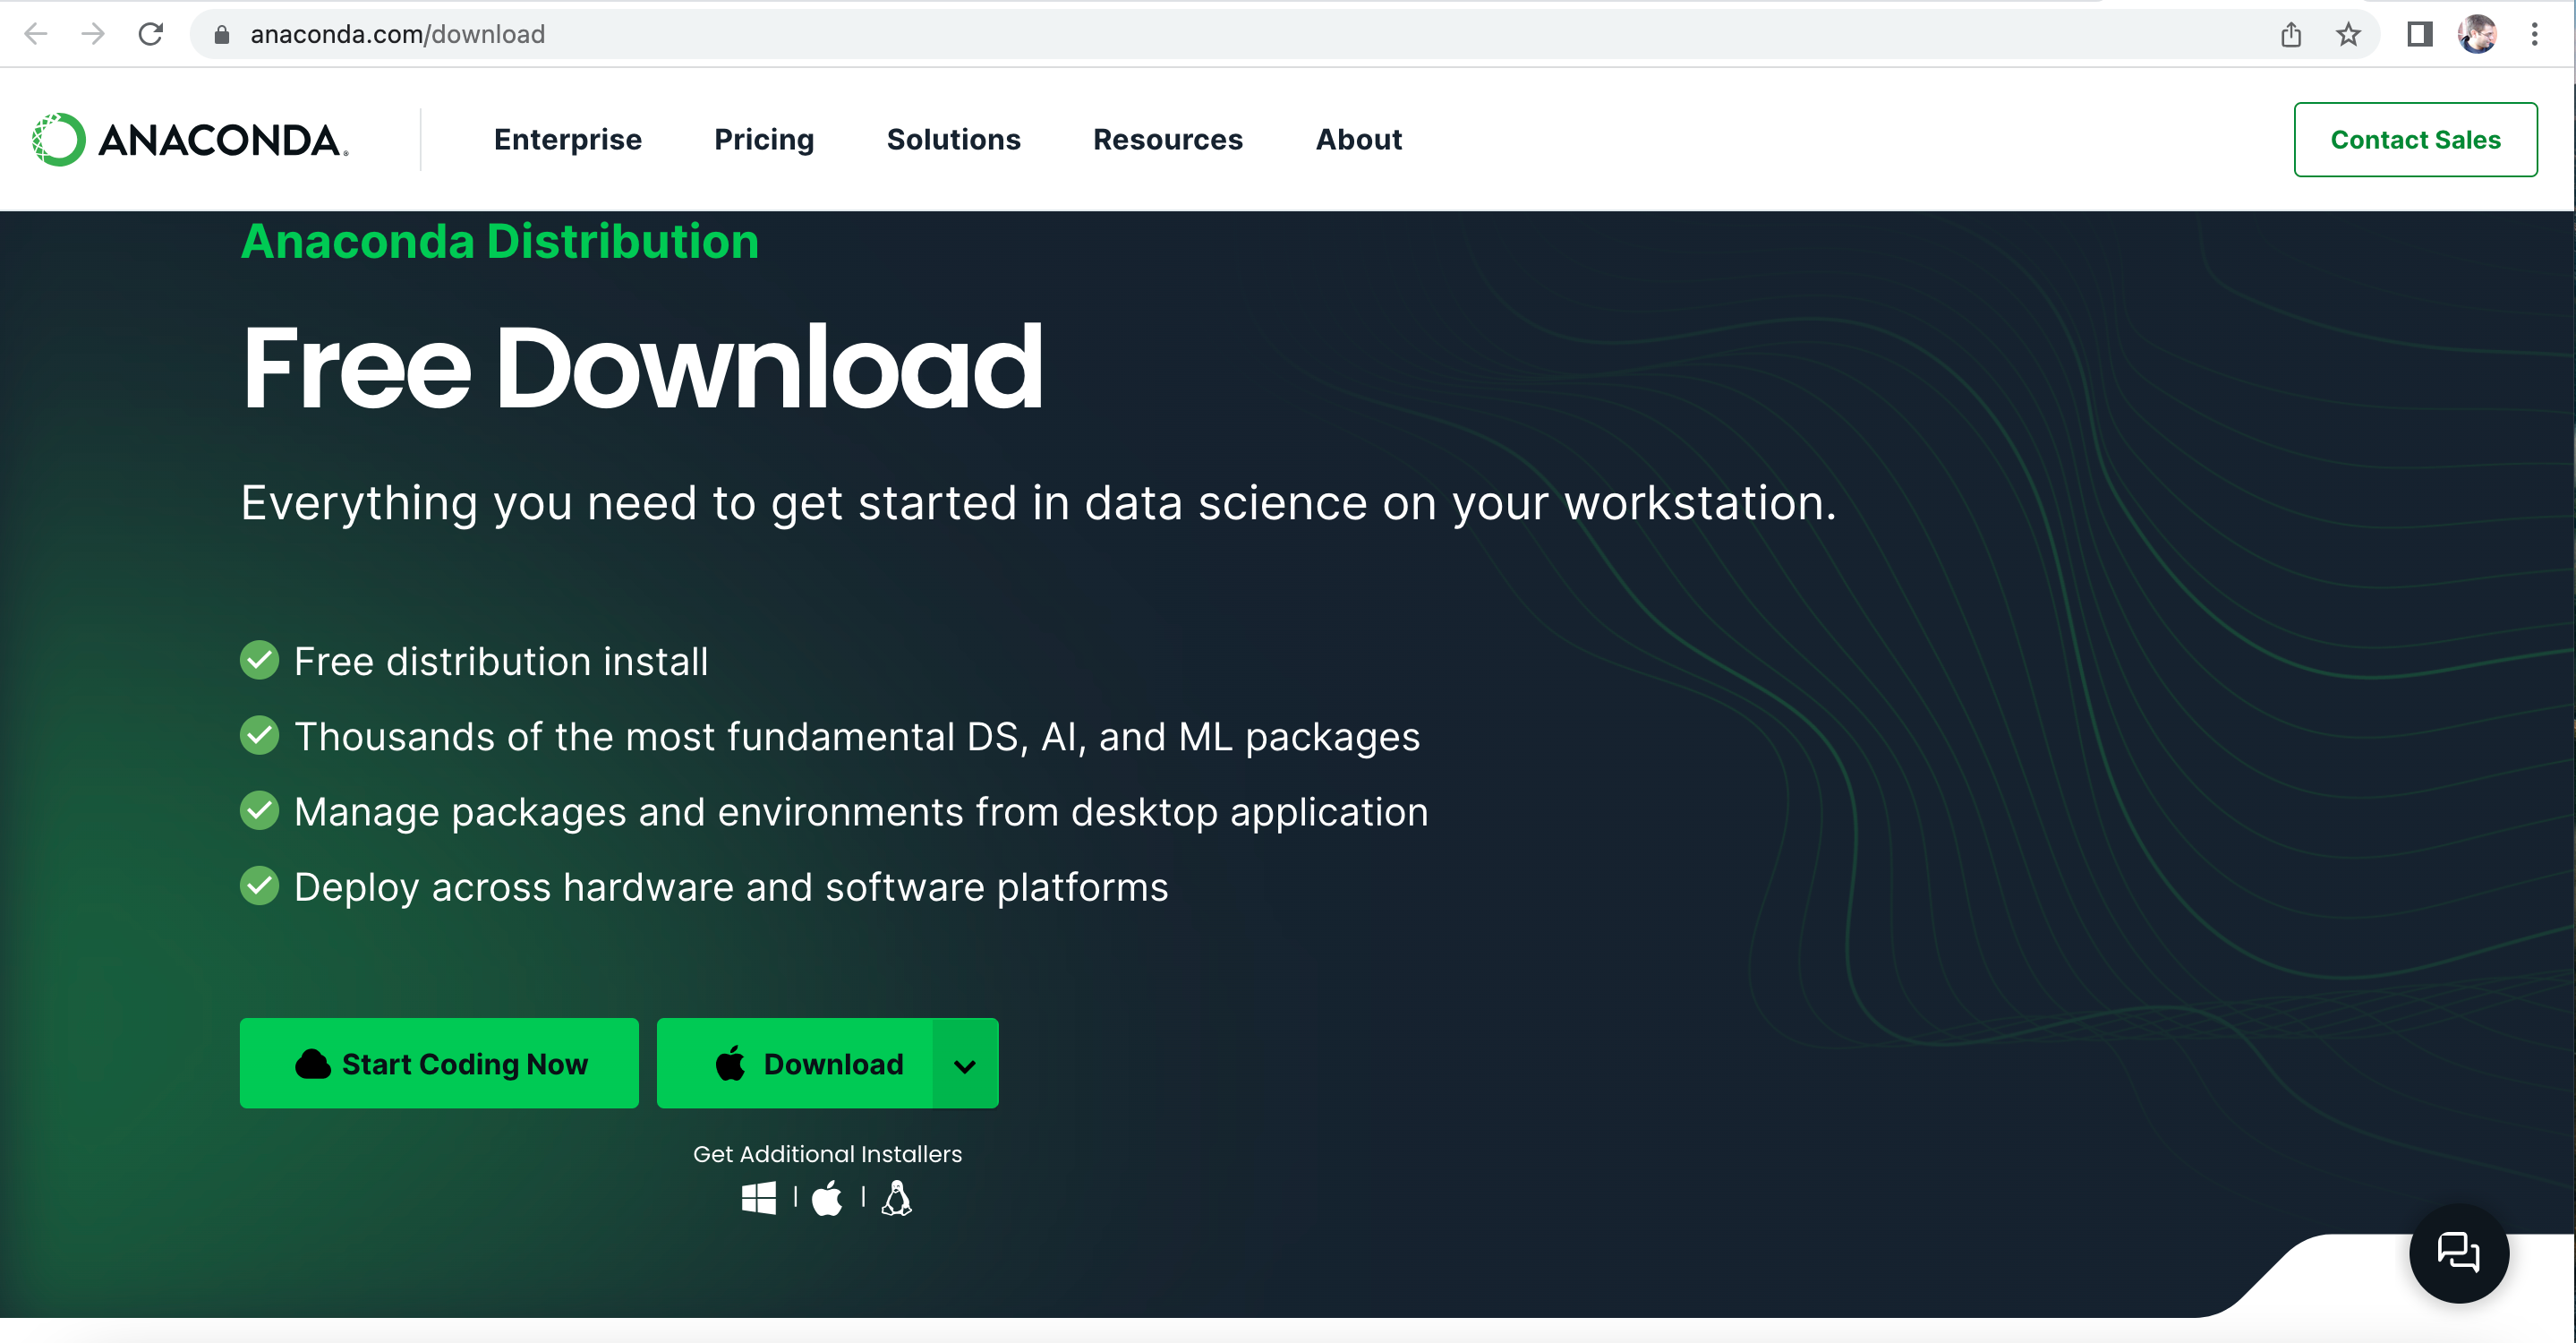
\includegraphics[scale = 0.1]{\pathtoimages/anaconda.png}
\end{center}
\end{frame}

\begin{frame}
\frametitle{Anaconda}

After you've installed and opened Anaconda, a screen like this will appear. You have several choices for IDEs. Spyder is useful for data analysis. Jupyter Notebook is popular for explanatory work, so students and teachers tend to use it. You can use any IDE.
\begin{center}
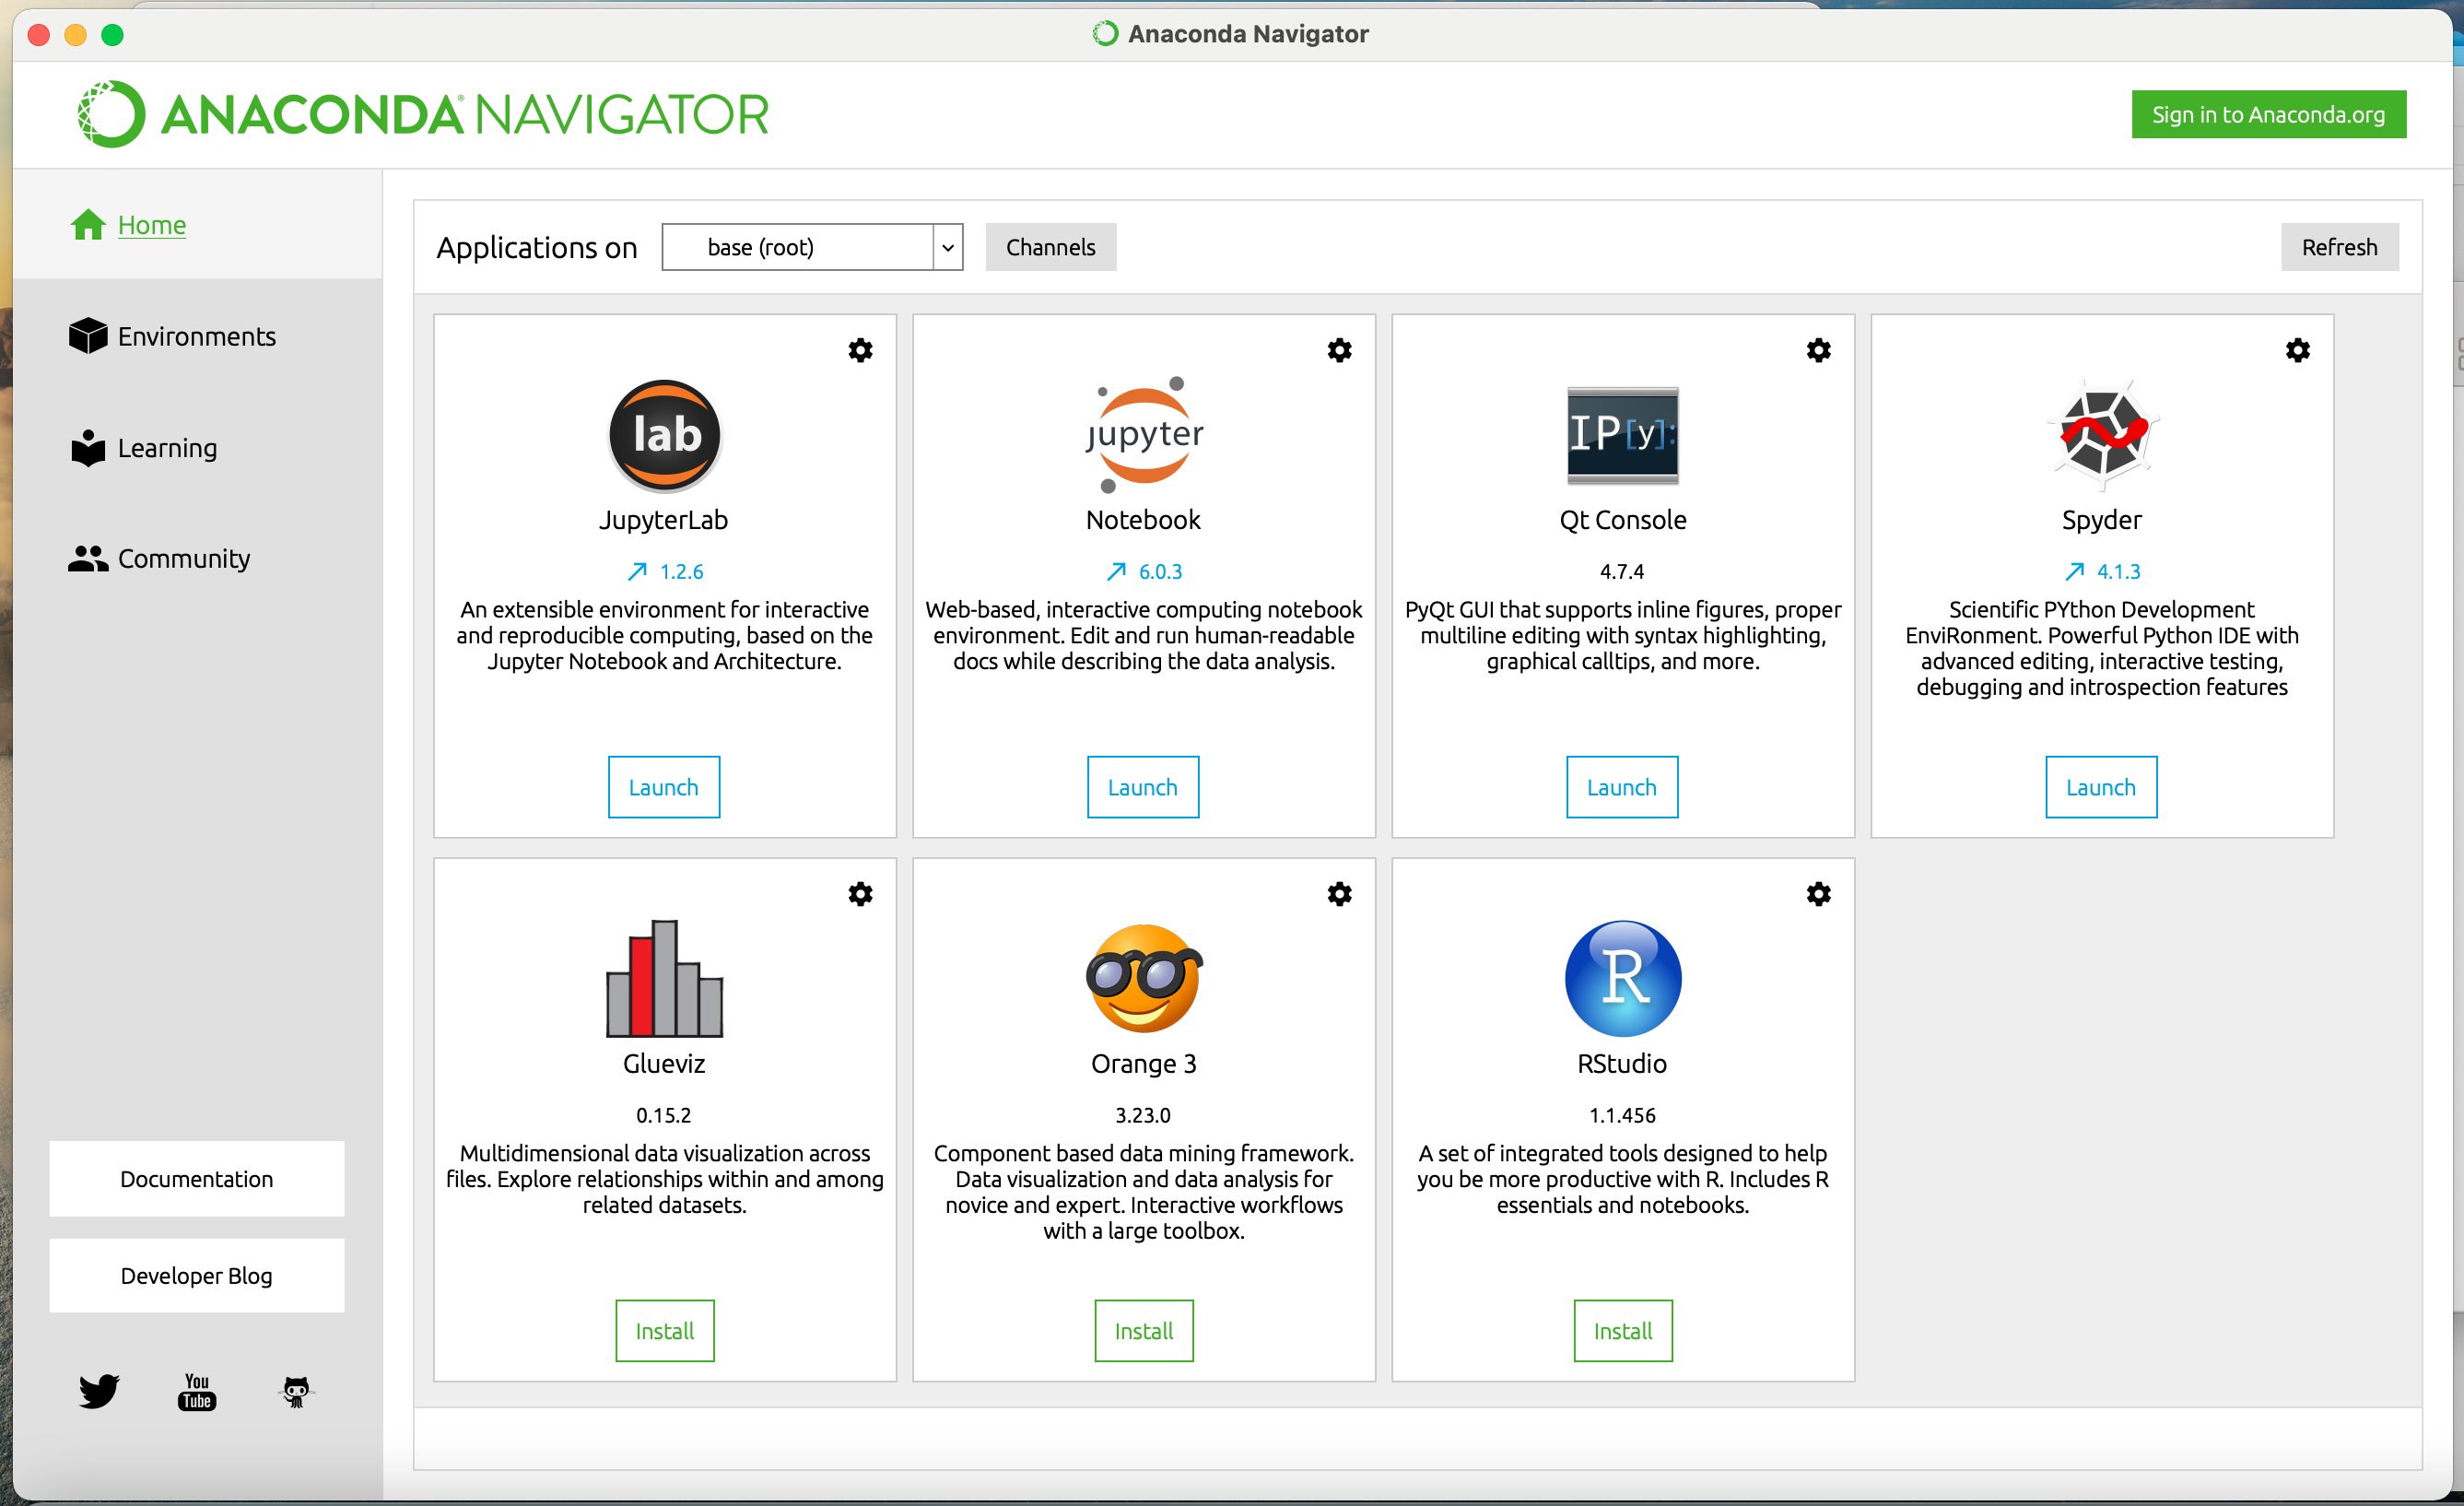
\includegraphics[scale = 0.1]{\pathtoimages/anaconda2.png}
\end{center}
\end{frame}

\frame{
\frametitle{Packages}

{
%\linespread{1.5}
Several popular modules (packages) are preinstalled in Anaconda. 
\begin{itemize}
\item {\it NumPy}:  Useful math functions.
\item {\it Matplotlib:} Graphing. Somewhat quirky syntax but very popular nonetheless. 
\item {\it SciPy}: Scientific computing functions.
\end{itemize}
}
}

\frame{
\frametitle{Package Installation} 
To install a new module, go into Terminal, and type 
\begin{center}
{\tt pip install \ldots}
\end{center}
In this example, I'm upgrading pandas. Your Terminal will probably look differently.
\begin{center}
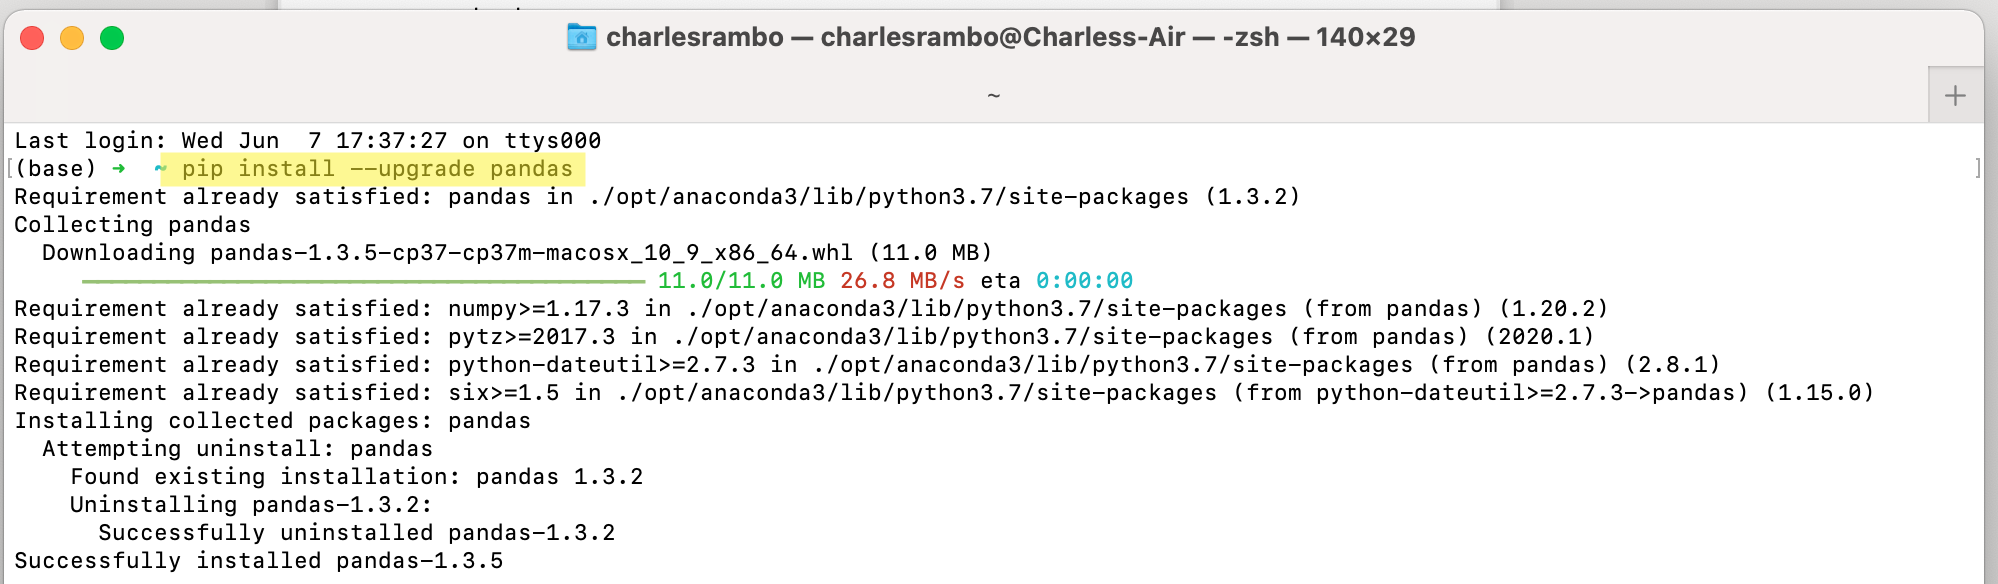
\includegraphics[scale = 0.2]{\pathtoimages/pip.png}
\end{center}
}

\begin{frame}[fragile]
\frametitle{Python Graphing Example}

\begin{example} 
Let $f(x) = x^2 + 1$. Use Python to graph $f$ on the domain $[-1, 2]$.
\end{example}

\begin{multicols}{2}
\begin{lstlisting}[language=Python]
# Import modules 
import numpy as np
import matplotlib.pyplot as plt

# These steps add style; less important

# Use latex
plt.rcParams['text.usetex'] = True

# Use Seaborn style
plt.style.use('seaborn')

# Define f
def f(x):
    return x**2 + 1

# Another option is to use a lambda function
# f = lambda x: x**2 + 1

# Get 100 x-values on [-1, 2]
x_vals = np.linspace(-1, 2, 100)

# Use list comprehension to get y-values
y_vals = [f(x) for x in x_vals]

# Automatically vectorized so this works too
# y_vals = f(x_vals)

# Generate the plot
plt.plot(x_vals, y_vals)

# Label the x-axis
plt.xlabel(r'$x$')

# Label the y-axis
plt.ylabel(r'$y$')

# Give the graph a title
plt.title(r'Graph of $y = x^2 + 1$')

# Save the figure
plt.savefig(path + r'ex0-1')

# Display the plot
plt.show()

\end{lstlisting}

\end{multicols}

\end{frame}

\begin{frame}
\frametitle{Python Graphing Result}
\begin{figure}
\centering
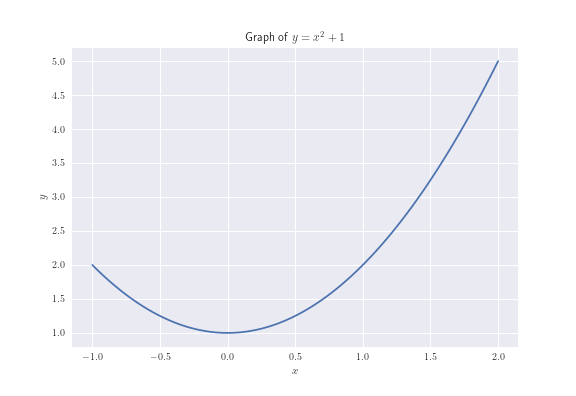
\includegraphics[scale = 0.5]{\pathtoimages/ex0-1.png}
\end{figure}
\end{frame}

\begin{frame}[fragile]
\frametitle{Python Optimization Example}
\begin{example}
Use Python to find the minimum of $f(x) = x^2 + 1$ on the interval $[-1, 2]$.
\end{example}

{\bf Solution.} From the graph on the previous page, we know that the minimum is $y = 1$ which occurs when $x = 0$. But let's use Python to verify this. Suppose the code above is still in our local environment. 

\end{frame}

\begin{frame}[fragile]
\frametitle{Python Optimization Example Cont.}

\begin{lstlisting}[language=Python]
# Import minimize from scipy
from scipy.optimize import minimize

# Define f
def f(x):
  return x**2 + 1
 
# Minimize function; set bounds equal to the domain
minimize(f, x0 = [1], bounds = [(-1, 2)])
\end{lstlisting}
}
The output is shown below. 
\begin{figure}
\centering
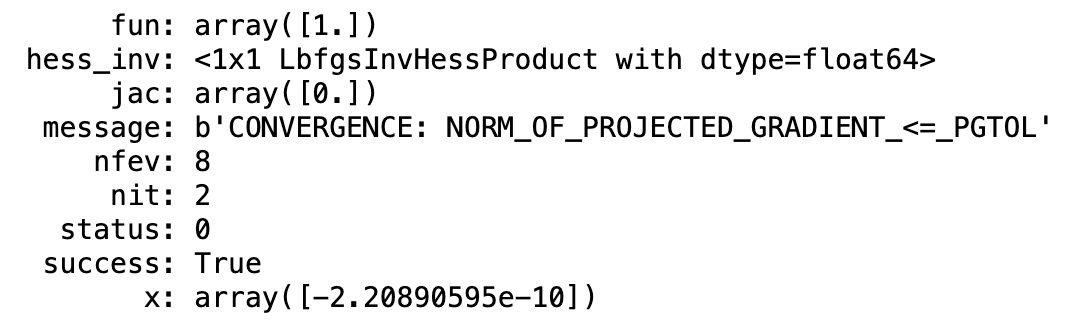
\includegraphics[scale = 0.5]{\pathtoimages/opt.png}
\end{figure}
\end{frame}

\end{document}